% Capítulo 3, Metodologia

\label{sec-tipo-pesquisa}

Este é um trabalho de pesquisa aplicada, de natureza experimental e quantitativa, com objetivos exploratórios e descritivos, e segue estratégia metodológica mista, organizada em duas linhas de trabalho. A primeira aplica um mapeamento sistemático da literatura \citep{petersen_mapping_2008} para identificar e classificar abordagens relacionadas a invariantes de estado de sessão, replicação assíncrona, tolerância a falhas, verificação formal por \emph{model checking} e mecanismos de decisão em sistemas distribuídos. A segunda é de pesquisa de projeto: o trabalho constrói e avalia, sob cenários parametrizados de falha, um conjunto de artefatos com recorte derivado dos achados da linha de mapeamento; os artefatos previstos são o modelo formal, o programa de carga instrumentado, o ambiente experimental em \emph{cluster} Infinispan e, em etapa posterior, o controlador heurístico. O relato dos resultados do mapeamento adota elementos do PRISMA 2020 \citep{prisma_2020}, em particular o fluxograma de seleção e a contabilização de itens por etapa. O guia em língua portuguesa de \citet{neiva_silva_revisao_sistematica_2016} apoia a operação do mapeamento. Por se tratar de um trabalho dividido em duas etapas, Trabalho de Conclusão de Curso~I e Trabalho de Conclusão de Curso~II, o presente texto reporta o protocolo, a execução inicial do mapeamento e os resultados parciais relativos à primeira etapa. 

\section{Mapeamento sistemático da literatura}
\label{sec-ms}
\revini{MET-02}\label{ap-protocolo-ms}\revfim{MET-02}

O mapeamento sistemático segue a sequência canônica proposta por \citet{petersen_mapping_2008}: define as questões de mapeamento, conduz a busca em bases bibliográficas, triagem os resultados por título e resumo, \revini{MET-55}classifica os trabalhos por palavras-chave extraídas dos resumos, recorrendo a outras partes do texto quando o resumo não basta, e, por fim, extrai e sintetiza os dados\revfim{MET-55}, e produz um esquema de classificação acompanhado de uma síntese descritiva. Esta seção sintetiza os elementos principais e relata a execução até a triagem inicial, correspondente ao escopo do presente Trabalho de Conclusão de Curso~I.

\section*{Pergunta central e questões de mapeamento}
\label{ap-questoes}

A pergunta central de pesquisa, formulada na Seção~\ref{sec-problema}, desdobra-se em sete questões de mapeamento. As questões investigam, respectivamente, quais invariantes de domínio do estado de sessão são tratados na literatura, quais modelos de falha são assumidos, quais mecanismos de replicação e reconciliação são empregados, quais abordagens e ferramentas de verificação formal são aplicadas, quais métricas e indicadores operacionais são reportados, quais mecanismos de decisão e adaptação são propostos, e quais plataformas e sistemas-alvo aparecem nos estudos empíricos. Cada questão está associada a um ou mais eixos temáticos do trabalho, conforme detalhado na Tabela~\ref{qd-qm}.

\begin{table}[h]
\captionsetup{type=table, name=Tabela}
\caption{Questões de mapeamento e eixos temáticos correspondentes}
\centering
\begin{tabular}{p{2.3cm}p{9cm}p{2.6cm}}
\hline
\textbf{Identificador} & \textbf{Questão de mapeamento} & \textbf{Eixos} \\
\hline
QM1 & Quais invariantes de domínio do estado de sessão são tratados na literatura? & sessão, replicação \\
QM2 & Quais modelos de falha são assumidos pelos trabalhos? & falhas, replicação \\
QM3 & Quais mecanismos de replicação e reconciliação são empregados? & replicação, IMDG \\
QM4 & Quais abordagens e ferramentas de verificação formal são aplicadas? & métodos formais \\
QM5 & Quais métricas e indicadores operacionais são reportados? & SLO, latência, observabilidade \\
QM6 & Quais mecanismos de decisão e adaptação são propostos? & autoadaptativo, controle \\
QM7 & Quais plataformas e sistemas-alvo são objeto dos estudos empíricos? & IMDG \\
\hline
\end{tabular}
\fonte{O autor}
\label{qd-qm}
\end{table}

\label{ap-bases-strings}A busca é executada nas bases ACM Digital Library, IEEE Xplore, Scopus e SpringerLink, escolhidas por reunirem as principais editoras e indexadores em Ciência da Computação. Conforme descrito na Seção~\ref{ap-selecao-validade}, a execução inicial empregou o agregador OpenAlex como porta única de acesso, e essa decisão deve ser complementada por execução manual via Portal de Periódicos CAPES na versão definitiva do protocolo. 

A pesquisa emprega seis \emph{strings} complementares, denotadas S1 a S6, organizadas por foco temático. Cada \emph{string} combina cláusulas \emph{OR} de termos-foco com cláusulas \emph{AND} de filtros transversais, e resulta de duas rodadas de calibração contra um conjunto-semente nomeado de referências-âncora. As versões finais das \emph{strings} são as seguintes:

\begin{itemize}[leftmargin=*]
    \item \textbf{S1, replicação, consistência e IMDG:} \texttt{((''in-memory data grid'' OR IMDG OR ''distributed cache'' OR ''key-value store'' OR ''session state'' OR ''session management'' OR ''distributed storage'' OR ''consistent hashing'' OR ''rebalancing'' OR ''state transfer'') AND (''consistency'' OR ''invariant'' OR ''convergence'' OR ''reconciliation'' OR ''replication'' OR ''CRDT'' OR ''eventual consistency'' OR ''session consistency''))}

    \item \textbf{S2, métodos formais aplicados a sistemas distribuídos:} \texttt{((''model checking'' OR ''formal verification'' OR ''formal specification'' OR ''temporal logic'' OR ''TLA+'' OR ''TLA'' OR Alloy OR SPIN OR Coq OR Isabelle OR ''bounded model checking'' OR ''probabilistic model checking'' OR ''theorem proving'') AND (''distributed'' OR ''replicated'' OR ''replication'' OR ''consistency'' OR ''concurrent'' OR ''protocol'' OR ''fault'' OR ''cache'' OR ''data grid''))}

    \item \textbf{S3, SLO, latência de cauda e observabilidade:} \texttt{((''SLO'' OR ''service level objective'' OR ''service level agreement'' OR ''tail latency'' OR ''p95'' OR ''p99'' OR ''percentile latency'' OR observability OR ''distributed tracing'' OR ''system monitoring'') AND (''distributed'' OR ''data grid'' OR ''cache'' OR ''key-value'' OR ''replicated'' OR ''scale'' OR ''latency''))}

    \item \textbf{S4, sistemas autoadaptativos e controle:} \texttt{((''self-adaptive'' OR autonomic OR ''MAPE-K'' OR ''feedback control'' OR ''control theory'' OR ''autoscaling'' OR ''auto-scaling'' OR ''autoscaler'' OR elasticity OR ''self-healing'' OR ''self-managing'' OR ''self-tuning'' OR ''adaptive control'') AND (''distributed'' OR ''cloud'' OR ''data grid'' OR ''key-value'' OR ''cache'' OR ''replicated'' OR ''fault'' OR ''service'' OR ''storage''))}

    \item \textbf{S5, fundamentos teóricos:} \texttt{((''consensus'' OR ''agreement protocol'' OR ''atomic broadcast'' OR ''linearizability'' OR ''failure detector'' OR ''impossibility'' OR ''network partition'' OR ''CAP theorem'' OR Byzantine OR Paxos OR Raft OR ''state machine replication'' OR ''vector clocks'' OR ''logical clocks'') AND (''distributed'' OR ''asynchronous'' OR ''fault-tolerant'' OR ''fault tolerance'' OR ''process'' OR ''replicat*''))}

    \item \textbf{S6, sessão como domínio:} \texttt{((''session management'' OR ''session state'' OR ''session invariant'' OR ''session lifecycle'' OR ''session token'' OR ''user session'' OR ''authentication state'' OR ''session fixation'' OR ''session hijacking'') AND (''distributed'' OR ''cluster'' OR ''replicat*'' OR ''cache'' OR ''data grid'' OR ''in-memory'' OR ''stateful'' OR ''security''))}
\end{itemize}

\section*{Critérios de inclusão e exclusão}
\label{ap-criterios}

Os critérios de inclusão filtram positivamente os trabalhos a considerar e são cinco. CI1 admite trabalho revisado por pares, obra clássica ou seminal, ou documentação técnica oficial. CI2 exige texto completo acessível. CI3 restringe os idiomas a português ou inglês. CI4 requer que o trabalho aborde, de modo substancial, pelo menos uma das questões de mapeamento. CI5 exige que o estudo trate como tema central sistemas distribuídos, replicação, consistência, falhas, verificação formal, observabilidade, controle adaptativo ou gerência de sessão.

Os critérios de exclusão definem motivos de remoção e são sete. CE1 elimina trabalhos com apenas resumo disponível. CE2 elimina duplicatas, mantida a versão mais completa do mesmo trabalho. CE3 elimina documentos técnicos comerciais sem revisão por pares e sem conteúdo técnico verificável. CE4 elimina trabalhos cujo foco está fora dos eixos relevantes. CE5 elimina idiomas distintos dos aceitos. CE6 elimina fontes sem revisão por pares quando usadas como base teórica principal; relatórios técnicos do tipo \emph{Jepsen} são admitidos apenas como literatura cinza de apoio empírico. \revini{MET-56}CE7 elimina itens anteriores a 1985, ano do resultado de impossibilidade do consenso assíncrono \citep{fischer_lynch_paterson_flp_1985}, ressalvada\revfim{MET-56} a manutenção dos estudos seminais desse período pela cláusula CI1. Pela cláusula de inclusão, mantêm-se os estudos seminais anteriores a 1985, ano do resultado de impossibilidade do consenso assíncrono \citep{fischer_lynch_paterson_flp_1985}.

\section*{Esquema de extração e classificação}
\label{ap-extracao}

Cada estudo primário incluído é caracterizado pelas oito dimensões a seguir, com as categorias previstas registradas para cada uma. As categorias podem ser refinadas após a etapa de leitura completa, caso achados recorrentes não previstos justifiquem o ajuste.

\begin{description}[leftmargin=*, style=nextline]
    \item[D1, modelo de consistência alvo:] forte; sequencial; causal; sessão; eventual; consistência eventual forte (CRDT); quórum.
    \item[D2, modelo de falhas assumido:] parada silenciosa; parada com recuperação; omissão; particionamento; bizantino; misto; não especificado.
    \item[D3, mecanismo de replicação e reconciliação:] síncrona com quórum; assíncrona com gravação por último escritor; assíncrona com resolução pela aplicação; CRDT; relógios vetoriais; consenso (Paxos, Raft); replicação por máquina de estado.
    \item[D4, abordagem ou ferramenta formal:] TLA+ com TLC; Alloy; SPIN; Coq; Isabelle; verificação probabilística de modelos; verificação limitada de modelos; sem método formal.
    \item[D5, validação empírica realizada:] em IMDG identificado; em outro sistema; em simulação; não-empírico.
    \item[D6, domínio de aplicação:] sessão ou autenticação; chave-valor genérico; banco de dados distribuído; mensageria; cache de aplicação; outro.
    \item[D7, métricas reportadas:] latência média ou de cauda (p95, p99); vazão; taxa de violação; tempo de recuperação; tempo de convergência; consumo de recursos; outras.
    \item[D8, tipo de mecanismo adaptativo:] nenhum; estático configurável; heurístico baseado em regras; MAPE-K; controle de realimentação clássico; aprendizado de máquina.
\end{description}

\section*{Procedimento de seleção e ameaças à validade}
\label{ap-selecao-validade}
\label{sec-ms-execucao}

O procedimento de seleção compreende identificação, triagem por título e resumo, e elegibilidade por leitura completa. \revini{MET-04}A identificação registra, por base, a \emph{string} aplicada, a data de execução e a quantidade de itens retornados. A triagem por título e resumo aplica os critérios de exclusão imediatamente verificáveis. A elegibilidade aplica a leitura completa, com registro do motivo de cada exclusão.\revfim{MET-04} Os números obtidos em cada etapa são reportados conforme o padrão PRISMA 2020 \citep{prisma_2020}. A execução inicial do mapeamento, correspondente às semanas 3 e 4 do cronograma do Trabalho de Conclusão de Curso~I, foi conduzida em 13 de maio de 2026 e utilizou o agregador OpenAlex como porta única de acesso às bases declaradas, em razão de restrições de acesso programático aos portais. Essa decisão é registrada como limitação metodológica do mapeamento sistemático. A Tabela~\ref{qd-prisma} sintetiza o fluxo nas três primeiras categorias e registra a etapa de Inclusão como em curso, dado que a classificação final dos estudos primários selecionados integra o Trabalho de Conclusão de Curso~II.

\begin{table}[h]
\captionsetup{type=table, name=Tabela}
\caption{Síntese do fluxo PRISMA 2020 do mapeamento sistemático até a etapa atual}
\centering
\begin{tabular}{p{8cm}r}
\hline
\textbf{Etapa PRISMA e subetapa} & \textbf{Quantidade de itens} \\
\hline
Identificação: itens recuperados pela união das \emph{strings} S1 a S6 & 8.669 \\
Identificação: itens removidos por duplicidade por DOI ou identificador & 1.586 \\
Triagem: itens em triagem após deduplicação & 7.083 \\
Triagem: itens aceitos por filtros básicos (tipo, idioma, ano) & 6.590 \\
Triagem: itens adicionados pelo conjunto-semente de calibração & 8 \\
Triagem: itens aceitos por título e resumo & 2.536 \\
Elegibilidade: itens selecionados para leitura completa & 165 \\
Inclusão: itens classificados nas oito dimensões D1 a D8 & em curso \\
\hline
\end{tabular}
\fonte{O autor}
\label{qd-prisma}
\label{tab-ms-execucao}
\end{table}

O relato do processo de seleção adota o modelo de fluxograma do PRISMA 2020, reproduzido na Figura~\ref{fig-prisma}, que organiza o fluxo de itens em três blocos sucessivos, denominados \emph{Identification}, \emph{Screening} e \emph{Included}, e reserva em cada etapa um campo para a contagem de registros e para os motivos de remoção. A figura apresenta o arcabouço em sua forma de modelo, com os campos de contagem ainda não preenchidos, dado que a versão povoada com os números de cada etapa, a contagem da etapa de Inclusão e o detalhamento dos motivos de exclusão (CE1 a CE7) por etapa será apresentada na monografia final, após a classificação integral dos 165 estudos primários selecionados. Os quantitativos já apurados até a etapa atual constam da Tabela~\ref{qd-prisma}.



\begin{figure}[htb]
\centering
\caption{Modelo de fluxograma PRISMA 2020 para o relato do processo de seleção de estudos.}
\label{fig-prisma}
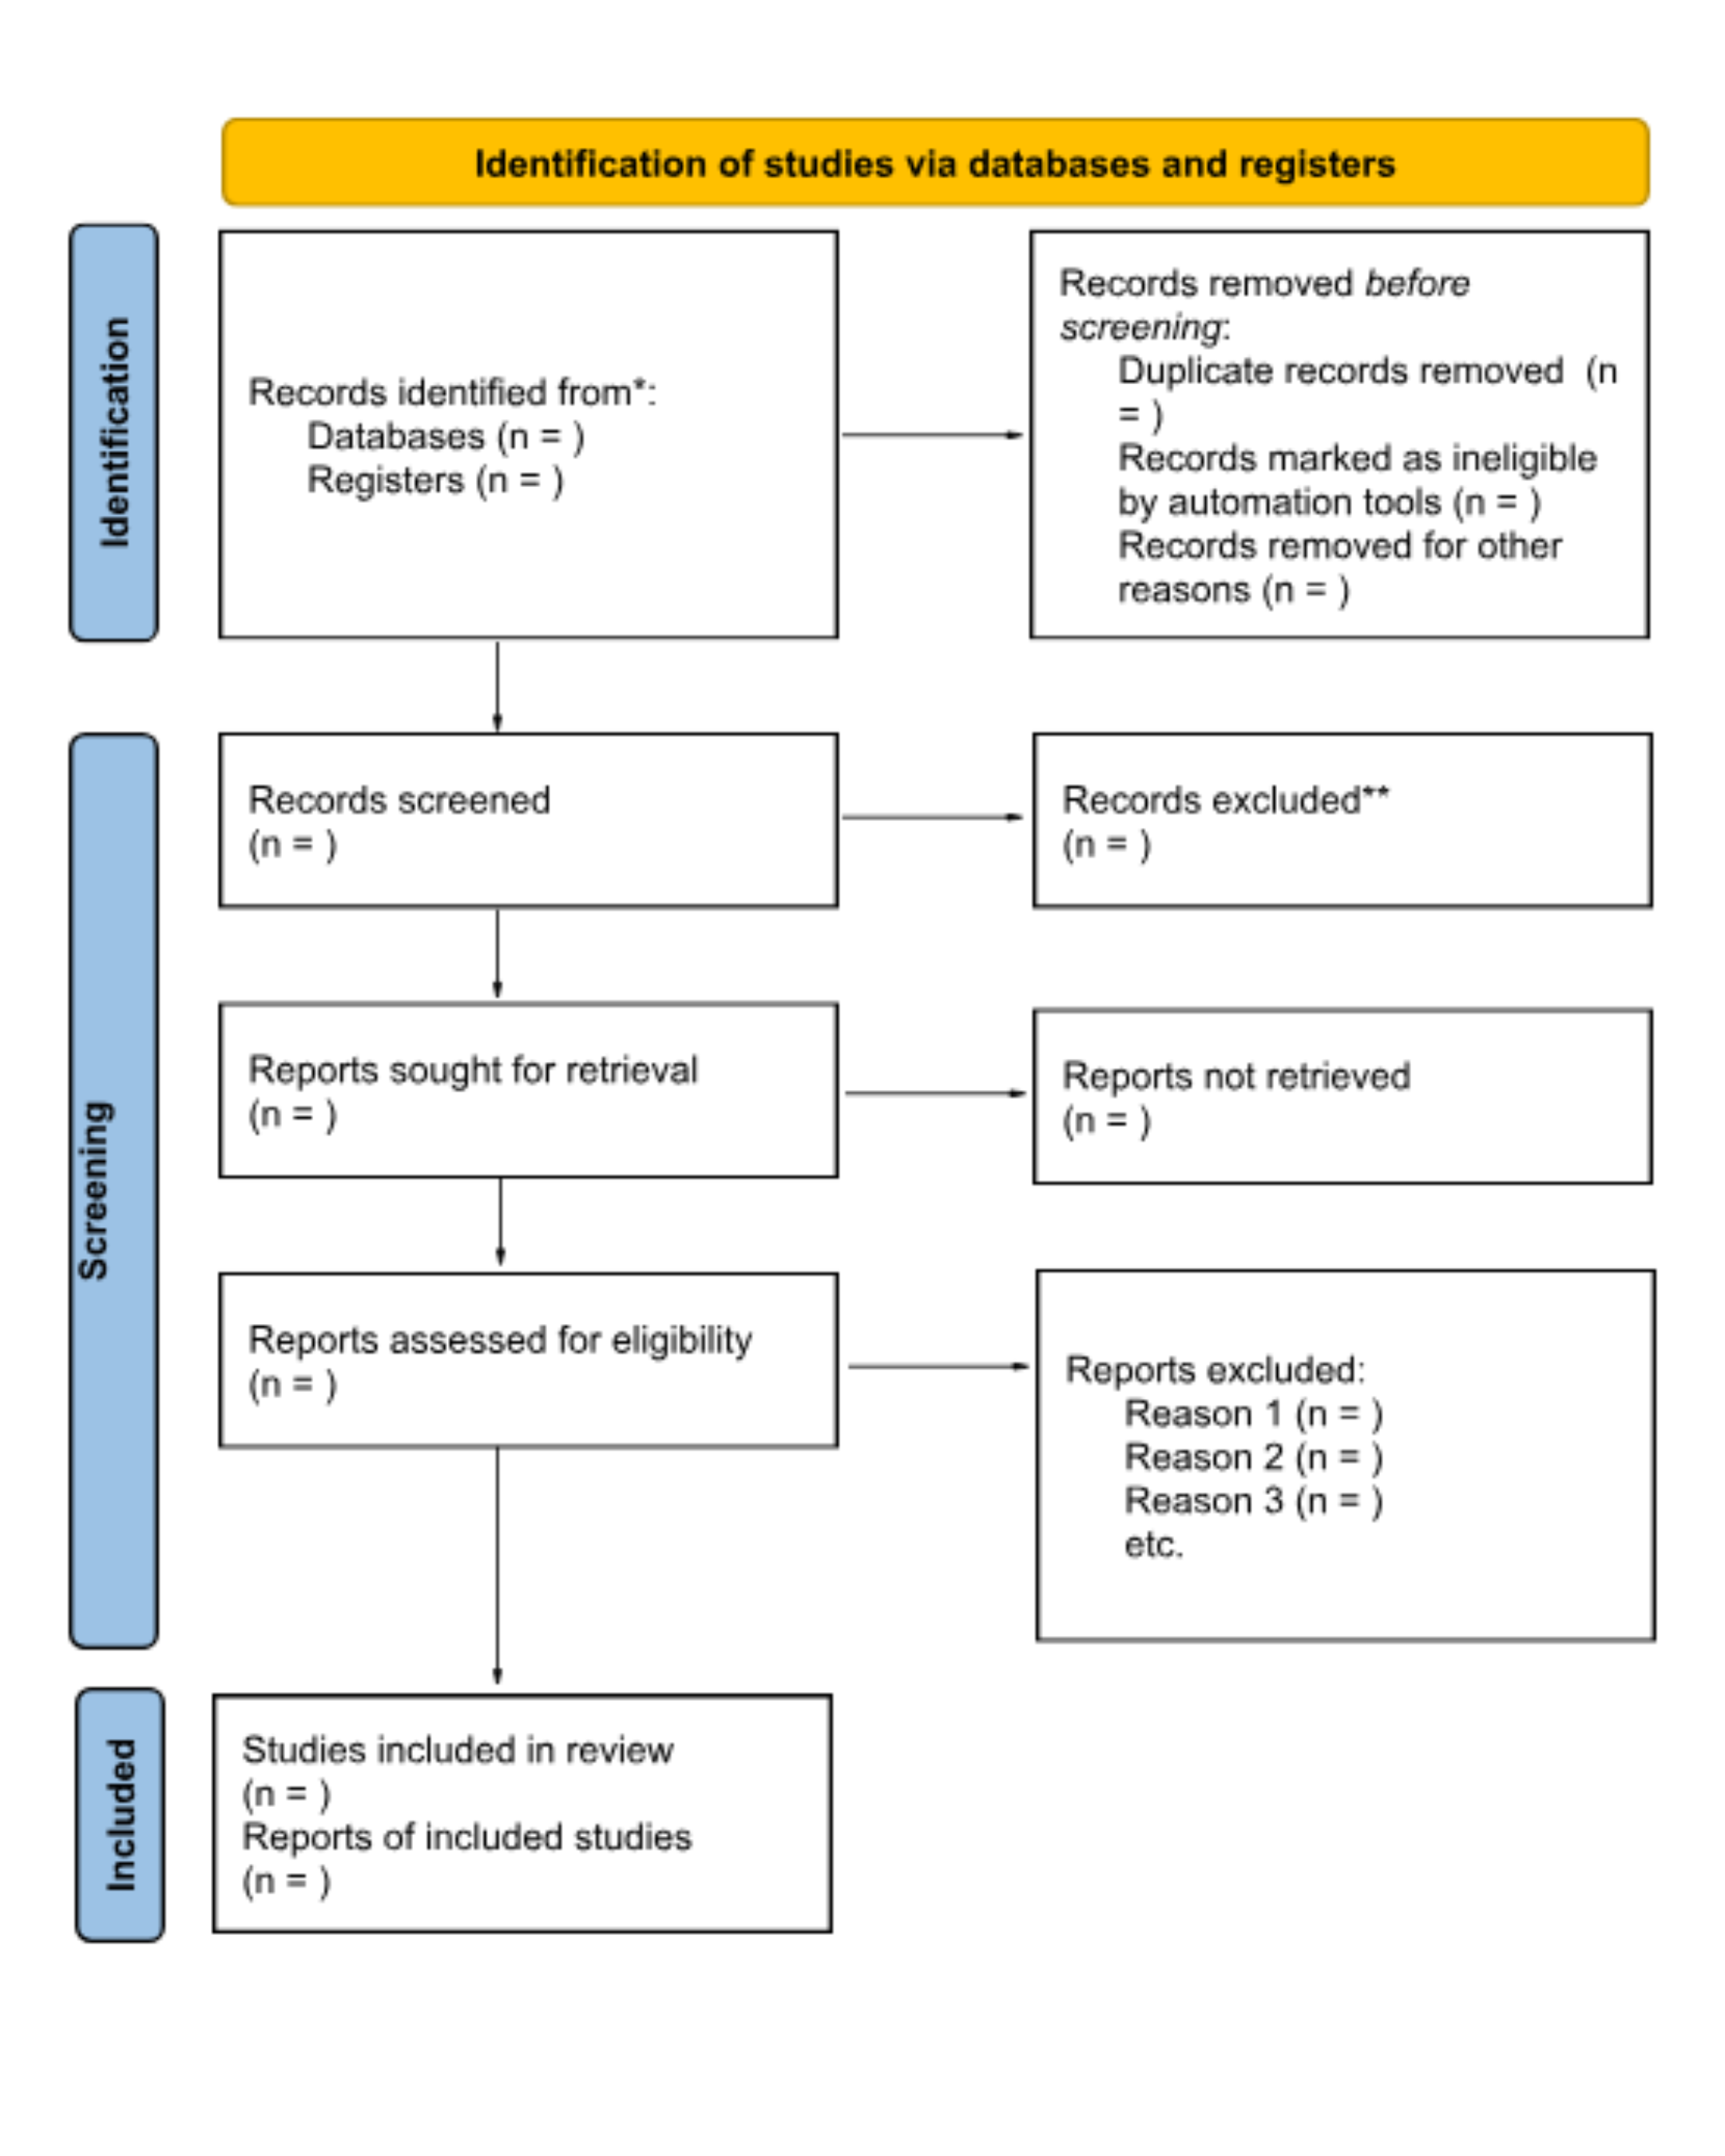
\includegraphics[width=0.9\textwidth]{figuras/prisma-fluxograma.png}
\fonte{\citeonline{prisma_2020}}
\end{figure}

São reconhecidas, ainda, cinco ameaças à validade do mapeamento. A primeira é a cobertura incompleta inerente ao conjunto de bases escolhidas, mitigada parcialmente pela amplitude do agregador empregado na execução inicial. A segunda decorre dos vieses de seleção e extração, mitigada pela documentação completa dos critérios e pela validação contra o conjunto-semente nomeado. A terceira reside em eventual subinclusividade ou superinclusividade das \emph{strings} de busca, mitigada pelas rodadas de calibração registradas na memória técnica do trabalho. A quarta é a datação dos resultados, registrada explicitamente em cada execução de busca. A quinta é a cobertura de literatura cinza, restrita conforme o critério CE6.

\section{Especificação formal e validação experimental}
\label{sec-frente-experimental}

A linha experimental reúne duas atividades acopladas. A primeira especifica formalmente o núcleo do protocolo de estado de sessão como um sistema de transições, com canal de replicação assíncrona abstrato, e verifica os invariantes declarados por \emph{model checking}. A segunda implementa e valida experimentalmente os mesmos invariantes em um \emph{cluster} Infinispan, com injeção parametrizada de falhas e instrumentação do programa de carga para detectar violações e medir percentis de latência. O recorte aplicado a ambas as atividades é derivado dos achados da linha de mapeamento. No escopo correspondente ao Trabalho de Conclusão de Curso~I, esta linha cobre a preparação do ambiente, a implementação do programa de carga, a especificação formal inicial do modelo (ainda sem falhas explicitamente modeladas) e a execução de \emph{baseline} experimental parcial sob um subconjunto dos cenários de falha previstos.  Os resultados parciais são reportados no Capítulo~\ref{cap-desenvolvimento}.

\section*{Escolha do ferramental de verificação}
\label{sec-escolha-ferramenta}

A verificação formal do núcleo do protocolo admite ferramentas de naturezas distintas, e a seleção pondera expressividade, custo de prova e ajuste ao recorte do trabalho. A análise relacional limitada por escopo com Alloy \citep{jackson_software_abstractions_2012} verifica invariantes estruturais sobre relações, mas opera sob limite de escopo e perde força na representação de um canal assíncrono com muitos passos de execução. O \emph{model checking} explícito de protocolos com SPIN e a linguagem Promela \citep{holzmann_spin_2004} é maduro para sistemas de processos comunicantes, porém opera em nível mais baixo e oferece menos expressividade para invariantes em teoria de conjuntos sobre os mapas que descrevem o estado de sessão. Os assistentes de prova como Coq e Isabelle provam propriedades sem limite de estados, mas exigem prova manual interativa, esforço desproporcional ao recorte do protocolo e ao cronograma das duas etapas. As abordagens empíricas para a mesma garantia, como testes baseados em propriedades, engenharia do caos e verificação a posteriori do tipo Jepsen \citep{bailis_kingsbury_network_2014}, validam o que o sistema executa, mas não certificam o que é possível no espaço de estados, e no presente trabalho já estão refletidas na vertente experimental descrita nesta seção.

A escolha recai sobre o conjunto TLA+ e TLC por quatro razões. A semântica de especificação de \citet{lamport_specifying_systems_2002} mapeia de forma direta os invariantes de segurança como propriedades de invariância, expressas pelo operador temporal $\square P$, que afirma que $P$ vale em todo estado da execução, e as propriedades de convergência sob quiescência declaradas na Seção~\ref{sec-invariantes}. O canal de replicação assíncrona é modelado como multiconjunto de mensagens com entrega não determinística, o que reproduz reordenação e atraso sem premissas de sincronia.  Há maturidade da linguagem e registro de aplicação industrial em sistemas de replicação \citep{newcombe_aws_formal_methods_2015, newcombe_aws_tla_2014}, o que reduz risco metodológico. Por fim, a cardinalidade reduzida do recorte (poucas identidades, sessões e réplicas, conforme o parâmetro T21 da Seção~\ref{sec-parametros}) mantém a verificação exaustiva do TLC tratável.  Dentro do mesmo ecossistema TLA+, o tradutor Apalache para verificação simbólica e o detector Must \citep{enea_must_2024} para protocolos assíncronos com falhas figuram como caminhos de escalabilidade reservados à etapa subsequente, quando o espaço de estados crescer com a inclusão explícita de falhas. 

\section*{Operações modeladas}
\label{sec-operacoes}

O protocolo de estado de sessão compreende sete operações sobre um par de mapas globais: o mapa $\sigma : \mathcal{S} \to \{\textsf{Valid}, \textsf{Invalid}(\textsf{reason})\}$, que associa a cada sessão $s$ seu estado lógico, e o mapa $\beta : \mathcal{U} \to \mathbb{N} \times \{\textsf{Free}, \textsf{Blocked}\}$, que associa a cada identidade $u$ o contador de tentativas e a marca de bloqueio.  As operações ficam definidas a seguir, com precondições e efeitos.

\textbf{O1, \emph{login}.} Cria nova sessão $s$ para uma identidade $u$ após validação de credenciais. Precondição: $\beta(u).\textsf{marca} = \textsf{Free}$. Efeito: $\sigma' = \sigma \cup \{s \mapsto \textsf{Valid}\}$, $\beta'(u).\textsf{counter} = 0$ (reposição implícita por sucesso). Caso a precondição falhe, a operação retorna o código de erro $\textsf{IdentityBlocked}$ sem alterar o estado. 

\textbf{O2, validação.} Operação de leitura que consulta o estado lógico atual de uma sessão. Sem efeitos sobre $\sigma$ ou $\beta$; retorna $\sigma(s)$ se $s \in \textsf{dom}(\sigma)$ e $\textsf{NotFound}$ caso contrário.

\textbf{O3, \emph{logout}.} Marca a sessão $s$ como inválida com motivo registrado. Efeito: $\sigma' = \sigma[s \mapsto \textsf{Invalid}(\textsf{logout})]$. A operação é idempotente: aplicar O3 duas vezes sobre a mesma sessão produz o mesmo estado.

\textbf{O4, incremento de tentativas falhas.} Adiciona uma unidade ao contador da identidade $u$ após autenticação falha. Efeito: $\beta'(u).\textsf{counter} = \beta(u).\textsf{counter} + 1$; se $\beta'(u).\textsf{counter} \ge \theta$, em que $\theta$ é o limiar de bloqueio (parâmetro do sistema), então $\beta'(u).\textsf{marca} = \textsf{Blocked}$ e $\sigma' = \sigma[s \mapsto \textsf{Invalid}(\textsf{blocked})]$ para toda sessão $s$ de $u$. 

\textbf{O5, reposição de tentativas.} Zera o contador da identidade $u$ após sucesso de \emph{login} dentro da janela. Efeito: $\beta'(u).\textsf{counter} = 0$, sem alterar a marca de bloqueio.

\textbf{O6, bloqueio administrativo.} Marca a identidade $u$ como bloqueada e invalida toda sessão ativa associada, independentemente do contador. Efeito: $\beta'(u).\textsf{marca} = \textsf{Blocked}$ e $\sigma' = \sigma[s \mapsto \textsf{Invalid}(\textsf{admin\_block})]$ para toda sessão $s$ de $u$.

\textbf{O7, desbloqueio.} Remove a marca de bloqueio e zera o contador. Efeito: $\beta'(u).\textsf{marca} = \textsf{Free}$, $\beta'(u).\textsf{counter} = 0$. Não recria sessões previamente invalidadas.

\revini{MET-13}Cada operação registra marcas de tempo de início e fim com precisão de nanossegundos, o servidor de conexão do cliente, o código de retorno e a chave, e alimenta as métricas de latência e a detecção de violações descritas na Seção~\ref{sec-metricas}.\revfim{MET-13}

\section*{Modelo de falhas}
\label{sec-falhas}

Quatro classes de falha são consideradas no escopo do Trabalho de Conclusão de Curso~I, cada uma parametrizada para reprodução experimental controlada. \revini{MET-14}As classes se enquadram na taxonomia de \citet{avizienis_taxonomy_2004}.\revfim{MET-14}

\textbf{F1, \emph{crash} silencioso de nó.} Um nó deixa de responder sem aviso prévio. Parâmetros: identificador do nó alvo, instante de início $t_\textsf{crash}$ medido em segundos desde o início da execução, e duração da indisponibilidade $\Delta_\textsf{crash}$ (com $\Delta_\textsf{crash} = \infty$ correspondendo a falha permanente). A reativação do nó, quando ocorre, expõe o cenário de recuperação (\emph{crash-recovery}) e ativa o procedimento de \emph{state transfer}. \revini{MET-15}A pilha de comunicação do \emph{cluster} tem dois detectores de falha: o FD\_ALL3, que suspeita de um nó depois de um intervalo sem mensagens de presença (T16), e o FD\_SOCK2, que suspeita assim que a conexão TCP com o nó se fecha. Para que a queda seja silenciosa e detectada pelo FD\_ALL3, a interface de rede do nó é desativada antes que o processo seja encerrado (Seção~\ref{sec-protocolo-rebaseline}).\revfim{MET-15}

\textbf{F2, partição de rede entre subconjuntos do \emph{cluster}.} O conjunto de nós é dividido em dois ou mais subconjuntos $\{P_1, P_2, \ldots\}$ tais que a comunicação entre subconjuntos distintos é descartada por um intervalo $[t_\textsf{part}, t_\textsf{part} + \Delta_\textsf{part}]$. Dentro de cada subconjunto, a comunicação permanece normal. Esta classe fica reservada para o Trabalho de Conclusão de Curso~II (Decisão 011, ponto 11), com F1 e F3 cobrindo o escopo experimental do Trabalho de Conclusão de Curso~I. \revini{MET-16}No experimento, um nó é isolado dos outros dois (minoria de um nó), e o fim do intervalo dispara a fusão das partições.\revfim{MET-16}

\textbf{F3, introdução de atraso e \emph{jitter} no canal.} O atraso aplicado a cada mensagem é amostrado de uma distribuição com média $\mu$ e desvio padrão $\sigma$ (parâmetros do cenário), com aplicação via \texttt{tc-netem} \citep{netem_manpage} no \emph{network namespace} de cada \emph{container}. A distribuição padrão adotada é lognormal, escolhida por aproximar a cauda longa observada empiricamente em redes reais; alternativas exponencial e uniforme ficam configuráveis para análise de sensibilidade. 

\textbf{F4, mudança de topologia que induz \emph{state transfer}.} A adição ou remoção controlada de um nó durante carga ativa o rebalanceamento do Infinispan e dispara transferência de segmentos entre nós, com janela de inconsistência transitória durante a propagação. Parâmetros: tipo de evento (entrada ou saída de nó), nó alvo, instante. F4 fica como ampliação opcional no Trabalho de Conclusão de Curso~I, com execução completa no Trabalho de Conclusão de Curso~II. 

Falhas bizantinas (mensagens corrompidas ou maliciosas) estão fora de escopo, \revini{MET-57}dado que o modelo de falhas deste trabalho supõe canal honesto\revfim{MET-57} (CE6 do protocolo do mapeamento, Seção~\ref{sec-ms}). Cenários multi-site (\emph{cross-site} replication) ficam reservados para a etapa subsequente do trabalho. 

\section*{Invariantes alvo}
\label{sec-invariantes}

O conjunto inicial de invariantes verificados no Trabalho de Conclusão de Curso~I tem seis elementos, declarados sobre os mapas $\sigma$ e $\beta$ definidos na Seção~\ref{sec-operacoes}, sobre o conjunto de réplicas $\mathcal{R}$, e sobre a sequência temporal de estados globais $\{S_t\}_{t \ge 0}$. Os quatro primeiros são propriedades de segurança e devem valer em todo estado alcançável. Os dois últimos são propriedades de convergência, próprias da consistência eventual, e valem sob hipótese de quiescência, ou seja, no estado em que não há operações em andamento e, cessadas as operações, as réplicas convergem para o mesmo valor. 

\textbf{I1, irreversibilidade da invalidação por \emph{logout}.} A partir do momento em que uma sessão atinge o estado inválido com motivo \emph{logout}, nenhum estado futuro pode ter essa mesma sessão como válida:
\[
\forall s \in \mathcal{S}, \forall t \ge 0: \quad \sigma_t(s) = \textsf{Invalid}(\textsf{logout}) \Rightarrow \forall t' \ge t: \, \sigma_{t'}(s) \ne \textsf{Valid}.
\]

\textbf{I2, consistência de bloqueio.} Enquanto uma identidade estiver marcada como bloqueada, nenhuma sessão associada pode ser validada como ativa:
\[
\forall u \in \mathcal{U}, \forall t: \quad \beta_t(u).\textsf{marca} = \textsf{Blocked} \Rightarrow \forall s \in \textsf{sessions}(u): \, \sigma_t(s) \ne \textsf{Valid}.
\]


\textbf{I3, monotonicidade local do contador.} Em cada réplica $r \in \mathcal{R}$, na ausência de reposição (O5) e desbloqueio (O7) entre dois instantes $t_1 < t_2$, o contador é não-decrescente:
\[
\forall u, \forall r, \forall t_1 < t_2: \quad \beta_{r, t_1}(u).\textsf{counter} \le \beta_{r, t_2}(u).\textsf{counter},
\]
restrito ao intervalo em que nenhuma operação O5 ou O7 sobre $u$ é aplicada em $r$.

\textbf{I4, unicidade do motivo de invalidação.} Uma vez fixado o motivo de invalidação de uma sessão, ele não é reescrito por outra causa:
\[
\forall s, \forall t: \quad \sigma_t(s) = \textsf{Invalid}(m) \, \land \, m \ne \bot \Rightarrow \forall t' > t: \, \sigma_{t'}(s) = \textsf{Invalid}(m).
\]

\textbf{I5, convergência do estado lógico (sob quiescência).} Após o cessar das operações e a entrega de todas as mensagens pendentes pelos canais (estado de quiescência $Q$), todas as réplicas observam o mesmo estado lógico para cada sessão:
\[
\textsf{quiescent}(Q) \Rightarrow \forall s, \forall r_1, r_2 \in \mathcal{R}: \, \sigma_{r_1}(s) = \sigma_{r_2}(s).
\]


\textbf{I6, convergência do contador (sob quiescência).} Sob a mesma hipótese, o contador converge entre réplicas:
\[
\textsf{quiescent}(Q) \Rightarrow \forall u, \forall r_1, r_2 \in \mathcal{R}: \, \beta_{r_1}(u).\textsf{counter} = \beta_{r_2}(u).\textsf{counter}.
\]


Os invariantes I3, I5 e I6 reconhecem explicitamente a separação entre estado local de cada réplica e estado lógico global; I5 e I6 derivam diretamente da Consistência Eventual Forte de \citet{shapiro_crdt_2011} aplicada aos tipos de dados subjacentes (registrador para $\sigma$, contador para $\beta.\textsf{counter}$). 

\section*{Métricas e critérios}
\label{sec-metricas}

A avaliação adota cinco métricas primárias coletadas por execução de cenário.

\textbf{Latência por operação.} Coletada como distribuição empírica, com cálculo de percentis p50, p95, p99 e p99,9 conforme prática consolidada para sistemas com cauda longa \citep{dean_barroso_tail_2013, google_sre_slo}. A coleta usa marcas de tempo de início e fim com precisão de nanossegundos, registradas pelo programa de carga, com agregação em janelas configuráveis para análise temporal.

\textbf{Taxa de violação por invariante.} Contabilizada como número de eventos detectados por unidade de tempo e por operação. A detecção segue dois caminhos (Seção~\ref{sec-arquitetura}): verificação imediata após cada operação para violações observáveis localmente (I1 a I4), e auditoria periódica em janelas de quiescência para violações de convergência (I5 e I6). Cada violação registrada inclui o invariante atingido, o estado relevante das réplicas e o histórico de operações que o produziu. 

\textbf{Tempo de recuperação.} Mede o intervalo $\Delta_\textsf{rec} = t_\textsf{base} - t_\textsf{fim-falha}$ entre o fim da injeção de uma falha (instante $t_\textsf{fim-falha}$) e o retorno da taxa de erro à linha de base (instante $t_\textsf{base}$, definido como o primeiro instante em que a taxa de erro permanece dentro de uma margem $\epsilon$ da pré-falha por uma janela de $W$ segundos).

\textbf{Tempo de convergência.} Mede o intervalo $\Delta_\textsf{conv}$ entre o fim da falha e o desaparecimento de divergências entre réplicas (detectado pela auditoria periódica reportando $\sigma_{r_1} = \sigma_{r_2}$ e $\beta_{r_1} = \beta_{r_2}$ para todo par $(r_1, r_2)$ de réplicas). 

\textbf{Taxa de erro.} Contabiliza as requisições que retornam código distinto de sucesso, sem implicar necessariamente violação de invariante. Inclui erros transitórios de comunicação, recusa por bloqueio, \emph{timeouts} e códigos específicos do cliente Hot Rod.

Métricas secundárias, coletadas via API e logs do Infinispan, incluem uso de CPU por nó, memória do \emph{heap}, número de eventos de rebalanceamento, número de mensagens RPC trocadas e tamanho da fila de propagação assíncrona \citep{infinispan_metrics}. A exposição segue o formato OpenMetrics \citep{openmetrics_spec}, com integração via JMX \citep{jmx_oracle}, e admite coleta por agente Prometheus opcional \citep{prometheus_docs}. 

Os critérios de comparação entre o \emph{baseline} estático e a configuração com o controlador heurístico, planejados para o Trabalho de Conclusão de Curso~II, exigem três condições simultâneas. \revini{MET-28}A primeira é redução estatisticamente significativa da taxa de violação, avaliada pelo teste não paramétrico de Mann-Whitney sobre as amostras de cada cenário ($\alpha = 0{,}05$).\revfim{MET-28} A segunda é manutenção das latências p95 e p99 dentro de margem aceitável, definida como degradação máxima de 10\% em relação ao \emph{baseline}, com intervalo de confiança de 95\%. A terceira é a auditabilidade das decisões do controlador: cada ação aplicada deve ser rastreável até a regra que a motivou, com registro do gatilho (observável + limiar), do estado anterior e do estado seguinte do controlador. Os três critérios devem ser cumpridos conjuntamente para que a configuração com controlador seja considerada melhoria sobre o \emph{baseline}. 

\section*{Parâmetros experimentais e fundamentação na literatura}
\label{sec-parametros}

A definição dos parâmetros operacionais do \emph{baseline} segue três princípios. O primeiro é a compatibilidade com a literatura de avaliação de \emph{key-value stores} e \emph{data grids} sob carga com cauda longa, exemplificada por \citet{jaiman_tailx_2020} no caso de Cassandra com YCSB e por \citet{decandia_dynamo_2007} no caso de Dynamo. O segundo é a aderência à configuração recomendada na documentação oficial do Infinispan \revini{MET-58}(\citeauthor{infinispan_docs_stable}, \citeyear{infinispan_docs_stable}, \citeyear{infinispan_metrics}, \citeyear{infinispan_tuning})\revfim{MET-58}, de modo que o experimento meça o comportamento do sistema em configuração próxima da praticada em produção. O terceiro é a proporcionalidade ao escopo do Trabalho de Conclusão de Curso~I (Decisão de recorte registrada na Seção~\ref{sec-frente-experimental}), que delimita o tamanho do \emph{cluster}, o conjunto de cenários de falha e o volume de operações para que o tempo de execução em \emph{Sem}~9 e 10 fique dentro da janela disponível.

{\scriptsize
\setlength{\tabcolsep}{2pt}
\begin{longtable}{p{0.6cm} p{3.0cm} p{3.5cm} p{2.0cm} p{2.2cm} p{2.7cm}}
\captionsetup{font=normalsize}
\caption{Parâmetros do \emph{baseline} experimental: faixa observada, fonte e valor adotado}
\label{tab-parametros-baseline}\\
\hline
\textbf{ID} & \textbf{Parâmetro} & \textbf{Faixa observada} & \textbf{Fonte} & \textbf{Valor adotado} & \textbf{Justificativa do recorte} \\
\hline
\endfirsthead
\multicolumn{6}{c}{\normalsize \tablename\ \thetable\ -- continuação} \\
\hline
\textbf{ID} & \textbf{Parâmetro} & \textbf{Faixa observada} & \textbf{Fonte} & \textbf{Valor adotado} & \textbf{Justificativa do recorte} \\
\hline
\endhead
\hline
\multicolumn{6}{r}{\footnotesize \emph{continua na próxima página}} \\
\endfoot
\hline
\endlastfoot
T1 & Modo de replicação & DIST\_SYNC, DIST\_ASYNC, REPL\_SYNC, REPL\_ASYNC & \citealt{infinispan_docs_stable} & DIST\_ASYNC (alvo) e DIST\_SYNC (controle) & objeto de estudo é replicação assíncrona \\
T2 & Número de nós & 3 mínimo; 16 em estudos comparáveis & \revini{MET-30}\citealt{jaiman_tailx_2020, yuan_simple_testing_2014} & 3 & escopo TCC-I; tolerância mínima a 1 falha; falhas de produção reproduzíveis com até 3 nós\revfim{MET-30} \\
T3 & \texttt{numOwners} & 2 (padrão); $>2$ aumenta durabilidade & \citealt{infinispan_tuning} & 2 & padrão da documentação \\
T4 & \texttt{numSegments} & 256 (padrão); $20 \times N$ para $N>20$ & \citealt{infinispan_tuning} & 256 & dentro da faixa padrão para $N=3$ \\
T5 & Tamanho do \emph{payload} & 1 KB típico de sessão; 1 KB--2 MB em estudos de cauda & \citealt{jaiman_tailx_2020} & 1 KB fixo & representativo de objeto de sessão \\
T6 & Distribuição de chaves & \revini{MET-50}Zipfian $\rho=0{,}99$ (YCSB); uniforme; \emph{latest}\revfim{MET-50} & \citealt{cooper_ycsb_2010, jaiman_tailx_2020} & Zipfian $\rho=0{,}99$ & expõe a cauda; comparável com a literatura \\
T7 & Mistura de operações & 50/50, 95/5, 100R, leitura-modifica-escrita & \citealt{cooper_ycsb_2010, jaiman_tailx_2020} & 50/50 (cenário S1) + 95/5 (cenário S2) & 50/50 modela \emph{session store} de escrita ativa; 95/5 isola comportamento de validação \\
T8 & Cardinalidade de chaves & 50\,000 em \emph{benchmarks} sintéticos; 20\,M em estudos de cauda & \citealt{jaiman_tailx_2020} & 100\,000 & forma cauda Zipfian; cabe em \emph{heap} de poucos GB por nó \\
T9 & Operações por execução & \revini{MET-51}$10^6$--$10^7$\revfim{MET-51} & \citealt{jaiman_tailx_2020} & $10^6$ & viabiliza p99,9 estável ($n=1\,000$ amostras na cauda) \\
T10 & Repetições por cenário & 5 em estudos comparáveis & \citealt{jaiman_tailx_2020} & 30 & conservador para testes não paramétricos \\
T11 & \emph{Warm-up} & \revini{MET-52}fases de \emph{load} e \emph{run} separadas em YCSB & \citealt{cooper_ycsb_2010}\revfim{MET-52} & 60\,s ou 10\,\% do total; descarte das primeiras 5\,\% das amostras & estabilização de JIT, alocadores e cache \\
T12 & Carga (alvo) & 75\,\% do pico medido & \citealt{jaiman_tailx_2020} & 75\,\% do pico do piloto sem falhas & evita saturação; expõe variabilidade \\
T13 & Percentis reportados & p95 e p99 (mínimo da indústria); p99,9 em \emph{key-value stores} & \citealt{dean_barroso_tail_2013, decandia_dynamo_2007, google_sre_slo} & p50, p95, p99 obrigatórios; p99,9 quando $n \ge 10^6$ & padrão da literatura; p99,9 é estatisticamente
fiável com o volume adotado \\
T14 & Duração por cenário & \revini{MET-53}não reportada (estudos fixam número de operações)\revfim{MET-53} & \citealt{jaiman_tailx_2020} & 10\,min sem falha; 30\,min com falha & inclui a janela de detecção (T16) e estabilização \\
T15 & MTU & 1500 (padrão); até 9000 (\emph{jumbo}) & \citealt{infinispan_tuning} & 1500 & infraestrutura em \emph{containers} sem \emph{jumbo} controlado \\
T16 & Detecção de falha (FD\_ALL3) & \revini{MET-54}\emph{heartbeat} 8000\,ms, \emph{timeout} 40000\,ms, padrão da pilha JGroups do servidor (conferido na configuração do \emph{cluster}) & O autor\revfim{MET-54} & padrões mantidos & reproduz produção; define duração mínima de F1 \\
T17 & Falha F1 (\emph{crash}) & nó silencioso; reentrada com \emph{state transfer} & \citealt{infinispan_docs_stable} & 1 nó; $\Delta_\text{crash}=60$\,s; reentrada ativa & \revini{MET-31}maior que o \emph{timeout} de T16; ativa convergência (I5, I6)\revfim{MET-31} \\
T18 & Falha F3 (atraso/\emph{jitter}) & \revini{MET-33}atraso com média, desvio e distribuição configuráveis & \citealt{netem_manpage} & \revini{MET-32}$+50$\,ms no p99 via \texttt{tc-netem}\revfim{MET-32} & valor de engenharia, sem fonte empírica; calibrável\revfim{MET-33} \\
T19 & Métricas coletadas & latência, vazão, \emph{hit ratio}, RPC, \emph{state transfer} & \citealt{infinispan_metrics} & M1--M7 (Seção~\ref{sec-metricas}) & mapeamento 1:1 com os medidores expostos \\
T20 & Endpoint de métricas & JMX; OpenMetrics & \citealt{infinispan_metrics} & OpenMetrics; Prometheus opcional & padrão atual da documentação \\
T21 & Espaço de estados (TLC) & \revini{MET-34}cardinalidades pequenas (2--3 por \emph{sort}) em verificações industriais; falhas de produção com até 3 nós & \citealt{yu_lamport_tla_modelchecking_1999, newcombe_aws_tla_2014, yuan_simple_testing_2014}\revfim{MET-34} & 2--3 identidades, sessões e réplicas & expõe entrelaçamento concorrente; \emph{model checking}
incremental \\
T22 & Análise estatística & Mann-Whitney/Wilcoxon; \emph{bootstrap} para IC de percentis & \revini{MET-35}\citealt{mann_whitney_1947, efron_tibshirani_bootstrap_1993}\revfim{MET-35} & Mann-Whitney por percentil; \emph{bootstrap} com 10\,000 reamostragens para IC 95\,\% & distribuições assimétricas de latência \\
\end{longtable}
}
\fonte{O autor, com base em \citet{cooper_ycsb_2010}, \citet{decandia_dynamo_2007}, \citet{dean_barroso_tail_2013}, \citet{google_sre_slo}, \citet{infinispan_docs_stable}, \citet{infinispan_metrics}, \citet{infinispan_tuning}, \citet{jaiman_tailx_2020},
\revini{MET-49}\revfim{MET-49}\citet{yu_lamport_tla_modelchecking_1999}\revini{MET-36}, \citet{newcombe_aws_tla_2014}, \citet{yuan_simple_testing_2014}, \citet{netem_manpage}, \citet{mann_whitney_1947} e \citet{efron_tibshirani_bootstrap_1993}.\revfim{MET-36}}

 A Tabela~\ref{tab-parametros-baseline} sintetiza a análise, com a faixa observada na literatura ou na documentação oficial, a fonte principal e o valor adotado, e a justificativa do recorte. A tabela explicita três escolhas que merecem comentário. A combinação $10^6$ operações por execução (T9) com 30 repetições por cenário (T10) decorre da necessidade de estimar p99 e, quando aplicável, p99,9 sob incerteza controlada: com $10^6$ amostras, o p99,9 dispõe de $10^3$ observações na cauda, \revini{MET-37}base para um intervalo de confiança \emph{bootstrap} \citep{efron_tibshirani_bootstrap_1993}. Com 30 repetições, comparações entre cenários por percentil podem ser feitas pelo teste de \citet{mann_whitney_1947}, sem hipótese de normalidade,\revfim{MET-37} condição necessária dada a assimetria das distribuições de latência observadas em sistemas com cauda longa. A escolha de Zipfian $\rho=0{,}99$ (T6) e mistura 50/50 (T7) reproduz o setup de \citet{jaiman_tailx_2020} e a definição de \emph{Workload~A} do YCSB, descrito por \citet{cooper_ycsb_2010} como ``\emph{session store recording recent actions}'', e portanto põe o experimento em registro comparável com o estudo de cauda em Cassandra. A escolha dos valores padrão de detecção de falha (T16) deixa o cenário F1 (T17) com duração mínima alinhada ao \emph{timeout} de 40\,s, condição necessária para que o evento de falha seja registrado pelo \emph{cluster} antes do encerramento da janela experimental. 

\section*{Carga sintética dos cenários S1 e S2}
\label{sec-carga}

\revini{MET-39}Os cenários S1 e S2 da linha T7 da Tabela~\ref{tab-parametros-baseline} sorteiam, a cada iteração de cada \emph{thread} do programa de carga, uma operação com pesos fixos. Em S1, os pesos são 50\,\% de validação (O2), 25\,\% de \emph{login} (O1), 10\,\% de \emph{logout} (O3), 10\,\% de incremento de tentativas falhas (O4) e 5\,\% de reposição de tentativas (O5). Em S2, os pesos na mesma ordem são 95\,\%, 3\,\%, 1\,\%, 1\,\% e 0\,\%. O \emph{login} abre uma tríade: quando ele é aceito, a mesma \emph{thread} valida e encerra a sessão recém-criada, e os três eventos entram no registro. As validações e os \emph{logouts} sorteados fora da tríade, chamados aqui de isolados, recaem sobre chaves de sessão escolhidas pela distribuição Zipfian de T6, no universo de chaves de T8.

Antes do aquecimento de cada execução, o programa esvazia os dois \emph{caches} do modo de replicação em uso, confere que ambos ficaram vazios e encerra a execução com código de erro próprio se isso não ocorrer. Cada \emph{thread} $t$ usa, no \emph{login}, oito identidades próprias, \texttt{user-}$t$\texttt{-}$k$ com $k = 0, \dots, 7$, tomadas em rodízio, que nunca recebem O4 nem O5. As operações O4 e O5 atuam sobre uma identidade separada por \emph{thread}, \texttt{lim-}$t$, de modo que o bloqueio por limite continua exercitado sem atingir as identidades de \emph{login}. As chaves lidas pelas operações isoladas existem no \emph{cache}, conforme o esquema de gerações descrito a seguir. O rodízio não consome os geradores da mistura nem o de chaves.

A versão da mistura adotada nas medições organiza as chaves de sessão em \emph{slots}. O sorteio Zipfian define o \emph{slot} $k$, e um vetor compartilhado entre as \emph{threads} guarda a geração corrente $g_k$ de cada \emph{slot}. Antes do aquecimento, uma fase de carga grava, para cada um dos $10^5$ \emph{slots}, a geração 0 como sessão já invalidada por \emph{logout} e a geração 1 como sessão válida, o que soma $2 \times 10^5$ entradas e fixa $g_k = 1$. A sessão do \emph{slot} $k$ pertence à identidade \texttt{user-}$((k-1) \bmod T)$\texttt{-}$(\lfloor (k-1)/T \rfloor \bmod 8)$, em que $T$ é o número de \emph{threads}, a mesma em todas as gerações do \emph{slot}. A validação isolada lê a geração corrente, exceto quando um sorteio de Bernoulli independente, com probabilidade $p = 0{,}05$, a desvia para a geração anterior. Esse desvio representa um cliente que ainda apresenta um \emph{token} antigo. O valor de $p$ é uma premissa de engenharia, declarada como tal, e não a medida de um serviço real. O \emph{logout} isolado toma uma trava da faixa do \emph{slot} ($k \bmod 1024$), invalida a geração corrente, que é a operação medida e registrada, grava como válida a geração $g_k + 1$ e só então avança $g_k$. Essa gravação de reposição não emite evento, não entra na latência medida e não passa pelo auditor. Se o \emph{logout} retornar erro, não há reposição nem avanço. Se a reposição falhar, a geração não avança, e as validações seguem sobre a sessão já invalidada até o próximo \emph{logout} do \emph{slot}.

O desenho tem três consequências declaradas. A fração de respostas \textsf{Invalid} entre as validações isoladas fica estacionária desde o primeiro evento, próxima de $p$ acrescida da corrida entre uma validação e um \emph{logout} do mesmo \emph{slot}. A reposição acrescenta ao \emph{cluster} uma escrita por \emph{logout} isolado, ausente do registro de eventos, em número próximo de 10\,\% das operações em S1 e de 1\,\% em S2. A trava serializa no cliente os \emph{logouts} isolados de uma mesma faixa de \emph{slot}, que portanto não concorrem entre si, e a espera pela trava fica fora da latência medida. Os critérios de estacionariedade foram fixados antes de qualquer execução dessa versão da mistura. A fração \textsf{Invalid} entre as validações isoladas pode diferir no máximo 1,0 ponto percentual entre o primeiro e o terceiro terço da janela de medição (critério C1) e deve ficar no intervalo $[4{,}5\,\%;\ 6{,}5\,\%]$ (C2). Com $n$ validações isoladas e $k$ leituras de \emph{token} antigo, a execução deve satisfazer $|k/n - 0{,}05| \le 3{,}2905 \sqrt{0{,}05 \cdot 0{,}95 / n}$ (C3), região de aceitação do teste de $H_0\colon p = 0{,}05$ ao nível de 0,1\,\% pela aproximação normal da binomial, aplicada somente quando $n \cdot 0{,}05 \cdot 0{,}95 \ge 100$, limite adotado por cautela diante da cobertura errática dessa aproximação \citep{brown_cai_dasgupta_binomial_2001}. As contagens de C3 lidas na saída do programa e no registro de eventos podem diferir em até quatro eventos, o número de \emph{threads}, por causa da fronteira da janela de medição. Execução fora dessas tolerâncias é recusada.

O \emph{logout} e a cascata de invalidação do bloqueio administrativo (O6) invalidam sessões por escrita condicional à versão lida. O programa lê a sessão com sua versão e a substitui pela versão invalidada somente se a versão não tiver mudado; em caso de conflito, relê a sessão e tenta de novo, até três tentativas. A primeira invalidação vence, e o motivo registrado não muda depois. Uma invalidação que perde a escrita condicional e relê a sessão já invalidada é contada como invalidação perdida e não altera o estado. Se a sessão continuar válida, com versão alterada, depois da terceira tentativa, a operação termina com o código \texttt{ERROR\_TRANSPORT}, e um contador próprio de conflitos esgotados separa esse caso dos erros de transporte na análise. Os \emph{caches} permanecem não transacionais. O servidor emite uma vez por processo o aviso \texttt{ISPN006010}, segundo o qual operações condicionais devem ser usadas com \emph{caches} transacionais porque, de outro modo, ``\emph{data inconsistency issues could arise under failure situations}''. O guia do cliente Hot Rod faz a mesma recomendação, para que no \emph{failover} as operações condicionais não fiquem parcialmente aplicadas, com entradas conflitantes em nós diferentes \citep{infinispan_hotrod_java_15}, e o guia de configuração adverte que a divisão do \emph{cluster} em partições pode causar perda ou inconsistência de dados qualquer que seja a estratégia de tratamento ou a política de \emph{merge} \citep{infinispan_configuring_15}. A configuração não transacional foi mantida porque a adoção de \emph{caches} transacionais mudaria o sistema medido. Por isso, uma violação de I4 ou uma invalidação perdida observada sob falha (queda de nó, partição ou fusão de partições) é tratada na análise como efeito do \emph{grid}, e não da aplicação.

O \emph{login} relê a identidade depois de gravar a sessão. Se a releitura encontrar a identidade bloqueada, o próprio \emph{login} invalida a sessão recém-gravada com o motivo de bloqueio administrativo, pelo mesmo caminho condicional da cascata, e retorna recusa por bloqueio. Essa dupla checagem fecha, em \texttt{DIST\_SYNC}, a corrida entre um \emph{login} e um bloqueio concorrente da mesma identidade: o \emph{login} escreve a sessão e lê a identidade, o bloqueio escreve a identidade e lê as sessões, e, com operações linearizáveis, ao menos um dos dois observa a escrita do outro. Em \texttt{DIST\_ASYNC}, a releitura pode encontrar uma réplica atrasada, e o que restar dessa corrida é medida do \emph{grid}. A releitura custa uma leitura a mais por \emph{login} aceito, incluída na latência medida, e vale em todos os cenários, para que o \emph{login} meça a mesma operação em todos eles.

O auditor aplica mais três regras à contagem de violações. Uma validação que lê sessão válida sob identidade bloqueada é classificada pelo instante de início da leitura da sessão, comparado com dois marcos do bloqueio (a confirmação da identidade bloqueada e o fim da cascata de invalidação). A leitura anterior à confirmação conta como concorrente, apenas para diagnóstico; a leitura entre a confirmação e o fim da cascata recebe o rótulo de janela de cascata; a leitura sob cascata interrompida por erro recebe o rótulo de cascata incompleta; e somente a leitura posterior ao fim da cascata é registrada como I2. Dentro de uma mesma operação, cada par formado por invariante e sessão é registrado no máximo uma vez para I1 e I4. Um bloqueio cuja cascata esgota as tentativas termina em \texttt{ERROR\_TRANSPORT} com a cascata parcial, e a contagem de invalidações perdidas inclui apenas a invalidação que perdeu a escrita condicional e releu a sessão invalidada. As tabelas de violação contam I1, I4 e I2 a partir do arquivo de violações de cada execução, e uma I2 só entra como violação quando a análise do rastro do cliente a classifica como real. Os rótulos de janela e de cascata incompleta e os contadores de leituras concorrentes são reportados à parte. A leitura de sessão válida sob identidade bloqueada sem marco de bloqueio deve ser nula em \texttt{DIST\_SYNC}. Em \texttt{DIST\_ASYNC}, uma leitura atrasada da identidade depois do desbloqueio produz esse caso por efeito do \emph{grid}, e a contagem é reportada sem servir de critério.

O registro de eventos distingue, na validação, as respostas \texttt{VALID}, \texttt{INVALID} e \texttt{NOT\_FOUND}, e, no \emph{logout}, a chave ausente (\texttt{NOT\_FOUND}) da invalidação concluída. Ao fim de cada execução, um verificador de sanidade lê esse registro, conta os desfechos por operação na janela de medição e emite veredito sobre a coerência entre os desfechos observados e a mistura declarada. O veredito é desfavorável se não houver \emph{login}, se a fração de \emph{logins} aceitos entre aceitos e recusados por bloqueio ficar abaixo de 0,95, se nenhuma validação retornar \texttt{VALID}, se mais de 5\,\% das validações encontrarem a chave ausente, ou se a fração de alguma operação sorteada se afastar mais de 2,0 pontos percentuais do peso nominal do cenário. Esses limiares são fixados no programa de carga antes do piloto e não são ajustados depois de observados os dados. Como a campanha não registra marcadores de fase, as regras se aplicam a todos os eventos da janela de medição, inclusive aos do intervalo sob falha.

O tipo de cada operação, a chave sorteada e a decisão de ler o \emph{token} antigo vêm de três geradores \texttt{java.util.Random} próprios de cada \emph{thread}, derivados da semente da execução, do índice $t$ da \emph{thread} e da repetição $r$ pela expressão $s = \textit{semente} + t + 1\,000\,003 \cdot r$. O gerador de chaves usa $s$ diretamente. Os outros dois combinam $s$ com um sal próprio por ou exclusivo ($\oplus$) e aplicam a função de mistura de 64 bits do gerador SplitMix \citep{steele_lea_flood_splitmix_2014}, na variante usada por \texttt{java.util.SplittableRandom} ($\textsf{mix64}$), de modo que as três sequências sejam distintas: o gerador da mistura recebe a semente $\textsf{mix64}(s \oplus \textsf{SAL\_MISTURA})$, e o do \emph{token} antigo, $\textsf{mix64}(s \oplus \textsf{SAL\_TOKEN})$. Duas execuções com a mesma semente produzem, em cada \emph{thread}, a mesma sequência de intenções, isto é, os mesmos tipos de operação, \emph{slots}, decisões de \emph{token} antigo e identidades de \emph{login}. A intercalação entre \emph{threads}, as respostas do \emph{grid}, as latências, o número de operações por \emph{thread} e o trecho exato coberto pela janela de medição não são reprodutíveis, porque dependem do tempo. Com mais de uma \emph{thread}, o registro de eventos de duas execuções com a mesma semente não coincide, e a reprodutibilidade vale por \emph{thread}.\revfim{MET-39}

\section*{Cenário S3: simulação do ciclo de vida de sessões}
\label{sec-carga-s3}

\revini{MET-40}Os cenários S1 e S2 sorteiam operações com pesos fixos e não contêm bloqueio administrativo nem afinidade entre cliente e nó, de modo que não exercitam a consistência de bloqueio (I2) nem a escrita feita em um nó isolado por partição. O cenário S3 simula uma aplicação web com os defeitos de uma aplicação real: o programa não repara estado, não reconcilia réplicas e não repete operações indefinidamente, e o experimento registra o que o \emph{data grid} entrega nessas condições. Três servidores de aplicação, cada um ligado a um único nó do \emph{cluster}, atendem usuários virtuais fixados a eles, como sob um balanceador com afinidade; um quarto cliente faz o papel de console administrativo. Cada usuário de um primeiro conjunto de identidades faz \emph{login}, valida a sessão a cada página com tempo de pensar aleatório e, ao fim, encerra a sessão ou a abandona, caso em que a aplicação a considera expirada por inatividade e a sessão permanece válida no \emph{grid}. Depois de um \emph{logout} confirmado, o usuário repete validações da sessão encerrada por alguns segundos, como quem usa o botão de voltar do navegador, o que exercita I1 e I4.

Um ator administrativo bloqueia, em intervalos aleatórios, uma identidade com sessão ativa e a desbloqueia depois de um tempo mínimo, o que exercita I2 com cascata de invalidação. Um segundo conjunto de identidades recebe tentativas falhas até o limite, com reposições ocasionais, e mantém o bloqueio por limite separado do administrativo. O cliente tem tempos-limite curtos e no máximo duas retentativas de aplicação, depois das quais a operação conta como falha percebida pelo usuário. As ações de cada usuário são agregadas em ações S3, com a latência percebida, que inclui as retentativas. Os tempos de pensar, as durações de sessão, os intervalos do administrador e os tamanhos dos conjuntos de identidades são premissas de modelagem, sem fonte empírica, e serão fixados no pré-registro da campanha que usar S3. O cenário S3 é o objeto da campanha com F2 e F4 sob carga e da avaliação do controlador (Seção~\ref{sec-avaliacao-controlador}), enquanto a nova medição de referência usa apenas S1 e S2.\revfim{MET-40}

\section*{Protocolo da nova medição de referência}
\label{sec-protocolo-rebaseline}

\revini{MET-41}A nova medição de referência (\emph{rebaseline}) mede os dois modos de replicação da linha T1 na mesma campanha e com o mesmo \emph{jar}: \texttt{DIST\_SYNC} como controle e \texttt{DIST\_ASYNC} como alvo. O protocolo é pré-registrado \citep{nosek_preregistration_2018} antes de qualquer execução e não admite ajuste depois de observados os dados. Uma mudança gera registro novo, que cita o anterior e explica o motivo. A matriz cruza os cenários S1 e S2, com a carga da Seção~\ref{sec-carga}, os dois modos e três condições (sem falha, F1 e F3), em dez repetições de 300\,s por célula, o que soma 120 execuções, sem o controlador. Cada execução usa quatro \emph{threads} e um \emph{cluster} de três nós com a imagem \texttt{quay.io/infinispan/server:15.0.21.Final}, recriado do zero antes da campanha, com quatro \emph{caches}: um de sessões e um de contadores em cada modo. O cenário S3 e as falhas F2 e F4 ficam fora da campanha.

A janela de medição de cada execução vai de +44\,s a +300\,s. O aquecimento ocupa os primeiros 30\,s, valor de $\max(30\,\text{s},\ 10\,\% \cdot 300\,\text{s})$, e a política de aquecimento descarta ainda 5\,\% do tempo restante, ou seja, 14\,s. As falhas são disparadas no nó \texttt{isn2} a +49\,s do início do aquecimento, cinco segundos depois do início da medição, e a execução cujo disparo caia fora do intervalo de +48\,s a +51\,s é recusada. F1 desativa a interface \texttt{eth0} no \emph{network namespace} de \texttt{isn2} e, em seguida, encerra o processo do nó com o sinal \texttt{SIGKILL} (\texttt{podman kill}), sem saída ordenada. Após 60\,s, o \emph{container} é reiniciado com \texttt{podman start}. O nó fica fora de cerca de +49\,s a cerca de +109\,s, intervalo maior que o \emph{timeout} de 40\,s do detector FD\_ALL3 (T16). A desativação da interface antes do encerramento impede que o FD\_SOCK2 perceba o fechamento das conexões e detecte a queda em poucos segundos. F3 aplica \texttt{tc-netem} na interface \texttt{eth0} de \texttt{isn2}, com atraso de 20\,ms e desvio de 13\,ms sob distribuição normal, por 251\,s, até o fim da execução.

A ordem de execução segue blocos completos aleatorizados. Cada uma das dez rodadas executa as doze células uma vez, em ordem sorteada por gerador com semente fixada no registro, de modo que a deriva do ambiente ao longo da noite se distribua entre as células e que uma interrupção preserve rodadas completas. Uma rodada piloto com as doze células precede a campanha e serve para verificar o orquestrador, os critérios e os tempos; seus dados não entram em resultado. A execução de índice $i$ usa a semente $50\,000 + 100 \cdot i$, e nenhum par formado pela semente da \emph{thread} e pela repetição se repete na campanha, no piloto ou nas reposições. As execuções rodam em máquina virtual Linux sob Hyper-V, sem coleta de uso de CPU durante a campanha.

Cada execução passa por critérios de recusa fixados antes do piloto. Antes da carga, os três nós precisam estar saudáveis há pelo menos 60\,s, sem rebalanceamento em curso e sem disciplina \texttt{tc-netem} residual, e os dois \emph{caches} precisam começar vazios. Depois da execução, exigem-se término normal do programa de carga, veredito favorável do verificador de sanidade, carga inicial completa, os critérios C1 a C3 da mistura e a confirmação de que a falha ocorreu como previsto. Nas células com falha, C1 e C2 usam como denominador apenas as validações isoladas com resposta \texttt{VALID} ou \texttt{INVALID}, e os erros são reportados à parte. Nas células sem falha, exigem-se também ausência de validação com \texttt{NOT\_FOUND}, ao menos 99\,\% de \emph{logins} aceitos e ausência de reposições com erro, de invalidações perdidas e de conflitos esgotados. Nas células com falha, esses valores são apenas reportados. Em \texttt{DIST\_SYNC} sem falha, qualquer registro de I1, I2 ou I4, leitura sem marco de bloqueio ou \emph{login} revertido pela dupla checagem interrompe a campanha para investigação. Em \texttt{DIST\_ASYNC}, essas contagens são objeto de medição e são reportadas. O aviso \texttt{ISPN006010} pode aparecer no máximo uma vez por processo de nó, e o total por nó não pode exceder o número de vezes em que o processo foi iniciado, regra que acomoda o reinício de \texttt{isn2} em F1. A campanha é interrompida automaticamente diante de duas recusas na mesma célula, de mais de seis recusas no total ou de falha de infraestrutura, e uma recusa isolada é reposta no fim da campanha com o próximo índice livre.

A unidade estatística é a execução. Para cada execução e operação, a análise calcula p50, p95 e p99 das latências registradas na janela de medição, pelo método do posto mais próximo, sobre os desfechos válidos de cada operação: \emph{login} aceito, validação com \texttt{VALID} ou \texttt{INVALID}, \emph{logout} concluído, incremento contabilizado e reposição de tentativas concluída. Os demais desfechos entram nas taxas de erro por código. O p99 só é calculado com ao menos 1\,000 eventos válidos da operação na execução, e o p99,9 só com ao menos 10\,000, sem contraste. Os contrastes comparam F1 e F3 com a condição sem falha, por cenário, modo e operação, e \texttt{DIST\_ASYNC} com \texttt{DIST\_SYNC}, por cenário, condição de falha e operação. A estimativa de cada contraste é a diferença entre as médias dos p99 por execução das duas células, com intervalo de confiança de 95\,\% por \emph{bootstrap} percentil \citep{efron_tibshirani_bootstrap_1993} com 10\,000 reamostragens de execuções, feitas com reposição e de forma independente em cada célula. O contraste só é estimado quando cada célula tem ao menos oito execuções aceitas. O teste de \citet{mann_whitney_1947} bilateral sobre os p99 por execução, com $\alpha = 0{,}05$, é secundário. Os intervalos são reportados sem correção para comparações múltiplas, com a contagem de comparações declarada, e nenhuma conclusão depende de uma comparação isolada no limite da significância.

\revfim{MET-41}

\section*{Estimativa de energia}
\label{sec-energia}

\revini{MET-42}A máquina virtual Hyper-V que hospeda o \emph{cluster} não expõe ao sistema convidado os contadores de energia do processador, de modo que a energia não pode ser medida, apenas estimada por modelo \citep{kansal_vm_power_2010}. O método previsto lê, a cada segundo, o tempo de CPU acumulado e a memória de cada \emph{container} Infinispan pela interface cgroup v2 \citep{linux_cgroup_v2}, o tempo de CPU do processo do programa de carga, que inclui o controlador, e o uso total de CPU da máquina virtual, com o tempo tomado pelo hipervisor (\emph{steal}) registrado à parte. O relógio dessas leituras é o mesmo dos marcadores de falha, o que permite recortar o consumo por fase da execução. A métrica principal é medida, e não estimada: tempo de CPU por mil operações bem-sucedidas em S1 e S2 e por mil ações S3 sem falha percebida, acompanhado do retrabalho, contado em retentativas e operações com erro por ação útil.

A conversão em energia usa o modelo linear de \citet{fan_power_provisioning_2007}, com a potência ociosa e a potência máxima tomadas da especificação do processador do hospedeiro. A estimativa é reportada em duas parcelas: a dinâmica, proporcional ao tempo de CPU, e a total, que inclui a parcela ociosa, cujo peso \citet{barroso_holzle_energy_proportional_2007} destacam. A razão entre potência ociosa e máxima varia em $\{0{,}3;\ 0{,}5;\ 0{,}7\}$ como análise de sensibilidade. As conclusões são apenas relativas, entre os braços de uma comparação, e nunca em joules absolutos. O método tem limitações declaradas: o tempo de CPU virtual não equivale ao trabalho do núcleo físico; memória, disco e rede não entram na conta; e reduzir a carga reduz o consumo por definição, razão pela qual a métrica é normalizada por operação útil e a vazão útil tem margem de não inferioridade na avaliação do controlador. Uma execução com \emph{steal} acima de 5\,\% do tempo fica fora da comparação de CPU.\revfim{MET-42}

\section*{Desenho da avaliação do controlador}
\label{sec-avaliacao-controlador}

\revini{MET-43}O pré-registro da avaliação do controlador heurístico, com os valores finais, precede qualquer execução. A comparação ocorre em \texttt{DIST\_ASYNC}, o modo alvo, com o cenário S3, e opõe dois braços que executam o mesmo código: no braço A, o controlador observa e decide sem atuar (modo \emph{shadow}); no braço B, ele aplica as decisões (modo \emph{active}). Assim, o custo de observação é o mesmo nos dois braços, e só a atuação difere. São quatro células: sem falha, para medir sobrecarga e acionamentos indevidos; F2 com o nó \texttt{isn3} isolado por 90\,s; F4 com perda de 20\,\% (severidade N3); e F1 sobre \texttt{isn2}. Cada célula recebe oito blocos pareados, e cada bloco contém uma execução de cada braço com a mesma semente de carga, em ordem sorteada e com o \emph{cluster} reiniciado entre execuções. Os três primeiros blocos funcionam como piloto e são aproveitados se o protocolo não mudar. Duas células em \texttt{DIST\_SYNC} (F2 e F4), com quatro blocos cada, servem de referência, sem pretensão de teste, para indicar se o efeito depende do modo. O total é de cerca de 80 execuções, estimadas em 16 a 27 horas de máquina.

O desfecho primário de cada célula é o p99 da latência percebida das ações S3, que inclui as retentativas, nas fases durante a falha e de recuperação, calculado por execução. Para cada bloco $b$, calcula-se $d_b = \ln(p99_B / p99_A)$, e a estimativa é a média dos $d_b$, reportada como razão. O intervalo de confiança primário de 95\,\% é o intervalo $t$ sobre os $d_b$ \citep{student_probable_error_1908}, com o \emph{bootstrap} sobre blocos como análise de sensibilidade \citep{efron_tibshirani_bootstrap_1993}. O teste é de permutação exata por troca de sinal dos $d_b$ (\citeauthor{fisher_design_experiments_1935}, \citeyear{fisher_design_experiments_1935}, seção 21; \citeauthor{good_permutation_tests_2005}, \citeyear{good_permutation_tests_2005}), com $\alpha = 0{,}05$ por célula; com oito blocos, há $2^8 = 256$ arranjos, e o menor valor-$p$ bilateral possível é $2/256 \approx 0{,}008$. Os desfechos secundários (p99 por operação, taxa de erro, falhas percebidas, violações de I1, I2 e I4, tempo de convergência e divergência persistente de I5 e I6, tempo de CPU e energia estimada) seguem o mesmo procedimento, com correção de \citet{holm_sequential_1979} para múltiplas comparações dentro da célula.
Como as contagens de violação podem ser nulas, a análise principal dessas contagens é a diferença de taxas entre os braços, e uma contagem nula é relatada como ``não observada em $N$ ações'', com limite superior de 95\,\% próximo de $3/N$ \citep{hanley_lippmanhand_zero_1983}, e nunca como ausência do fenômeno.
A vazão útil, em ações S3 sem falha percebida por segundo, entra como critério de não inferioridade: o limite inferior do intervalo de 95\,\% da razão entre os braços deve ficar acima de $1 - \delta$, com $\delta = 10\,\%$. Esse critério impede que o controlador melhore a cauda apenas por reduzir a carga. A rastreabilidade, terceiro critério da Proposta, permanece: cada decisão grava os sinais, os limiares em vigor, a regra aplicada e o perfil resultante. Os limiares do controlador serão calibrados com dados da campanha com o cenário S3, por regra fixada antes de ver esses dados, e as execuções de calibração não entram na avaliação.\revfim{MET-43}

\section*{Trabalhos correlatos}
\label{sec-trabalhos-correlatos}

Esta seção apresenta os seis estudos de maior aderência ao desenho proposto, identificados entre os 165 itens selecionados pelo mapeamento para leitura completa. A descrição de cada um indica o que o trabalho realiza e o que o presente trabalho aproveita ou como dele se diferencia. A classificação integral dos estudos primários pelas dimensões D1 a D8 do esquema de extração, com o posicionamento sistemático em relação a cada agrupamento, integra a etapa inicial do Trabalho de Conclusão de Curso~II, conforme o Apêndice~\ref{ap-plano-tcc2}. A apresentação segue ordem temática, da verificação formal de protocolos à consistência sob monitoramento, à latência de cauda orientada a SLO e à autoadaptação por realimentação.

No eixo da verificação formal, \revini{MET-59}\citet{newcombe_aws_tla_2014} e \citet{newcombe_aws_formal_methods_2015}\revfim{MET-59} relatam a adoção de TLA+ pela Amazon Web Services para verificar protocolos de replicação, entre eles componentes do DynamoDB, com identificação de defeitos sutis antes da entrada em produção. O estudo legitima o método central deste trabalho, especificação em TLA+ e verificação por TLC, e fundamenta a prática de cardinalidades pequenas no espaço de estados, registrada como parâmetro T21 na Seção~\ref{sec-parametros}. A diferença está no domínio e no escopo: aqui o objeto é o estado de sessão sob recorte acadêmico, e a especificação formal é acoplada a um controlador heurístico em tempo de execução.

Ainda na verificação formal, \revini{MET-60}Must oferece uma interface de concorrência com vários modelos de comunicação, verifica os programas por redução parcial de ordem dinâmica e foi aplicada a sistemas de produção, como \emph{logs} replicados e protocolos de transação distribuída \citep{enea_must_2024}.\revfim{MET-60} A diferença é o ponto de partida: o núcleo sem falhas é tratado com TLA+/TLC, e Must figura como caminho de escalabilidade reservado ao Trabalho de Conclusão de Curso~II, quando as falhas forem modeladas de forma explícita. 

Para fechar o eixo formal, \citet{nair_safety_distributed_2020} provam a segurança de invariantes de objetos de alta disponibilidade por raciocínio composicional e local sob concorrência. O resultado liga os invariantes de convergência deste trabalho, I5 e I6, derivados da Consistência Eventual Forte dos CRDT, à literatura de prova formal de segurança. A diferença é metodológica: aqui a garantia provém de \emph{model checking}, com exploração exaustiva e produção de contraexemplos, em vez de prova dedutiva, e o alvo são invariantes específicos de sessão, I1 a I6.

Considerando consistência sob monitoramento, \citet{nguyen_weaker_consistency_2019} constituem o estudo de maior proximidade com o desenho proposto. Os autores combinam consistência relaxada, monitoramento e recuperação em armazenamentos chave-valor: o projetista identifica um predicado de correção $P$ sobre o estado distribuído, executa o protocolo sobre um armazenamento com consistência eventual ou causal, instrumenta a execução com um monitor que verifica $P$ por detecção de predicados distribuídos e aciona a reversão a um estado que satisfaz $P$ quando há violação. A avaliação sobre Voldemort, conduzida em instâncias EC2 da Amazon Web Services, registra vazão de 50\% a 80\% maior que a da consistência sequencial, custo de monitoramento tipicamente abaixo de 4\% e detecção de mais de 99,9\% das violações em menos de 50 milissegundos em redes regionais e em menos de 3 segundos em redes globais; os autores discutem ainda o caso em que reversões frequentes inviabilizam o progresso da aplicação. \revini{MET-46}A taxa de detecção acima foi medida em cenário projetado para provocar violações frequentes. Para o caso de reversões frequentes, os autores propõem mecanismos alternativos, como adiamento da resolução de violação ou avanço sob consistência mais restrita por janelas curtas.\revfim{MET-46} Este trabalho desloca a verificação formal a montante da execução, ou seja, antes de o sistema entrar em operação, no nível do modelo formal, com TLA+/TLC produzindo contraexemplos a priori; o controlador é heurístico e externo ao \emph{data grid}, atua sobre um conjunto finito de perfis com histerese, em vez da reversão reativa da camada de dados, e o estudo de caso é a gerência de sessão, com invariantes I1 a I6 derivados de fontes normativas \revini{MET-48}\citep{nist_sp_800_63b4_2025, owasp_session_mgmt_cheatsheet}\revfim{MET-48}.

Sobre latência de cauda orientada a SLO, \citet{jaiman_tailx_2020} propõem o TailX, escalonador de consultas \emph{multiget} heterogêneas para reduzir a latência de cauda em armazenamentos chave-valor, avaliado sobre Cassandra. O estudo fundamenta a adoção da cauda, percentis p95 e p99, como métrica primária deste trabalho e embasa vários valores do \emph{baseline} na Tabela~\ref{tab-parametros-baseline}, entre eles a distribuição Zipfian, a mistura de operações e o volume por execução. A diferença é o ponto de atuação: o TailX intervém no escalonamento das consultas, enquanto este trabalho atua sobre políticas e parâmetros de configuração em tempo de execução, por meio de um controlador heurístico, e amarra a latência à correção dos invariantes.

No eixo da autoadaptação, \citet{liu_onlineelastman_2017} apresentam o OnlineElastMan, gestor de elasticidade proativo e autotreinado para serviços de armazenamento em nuvem, orientado a SLO. \revini{MET-61}O estudo representa a adaptação por realimentação sobre métricas observadas.\revfim{MET-61} A diferença é a natureza do mecanismo: o controlador deste trabalho é heurístico, baseado em regras com histerese e portanto auditável, opera sobre um conjunto finito de perfis pré-definidos e responde a violações de invariantes e à cauda de latência, em vez de autoescalar por modelo aprendido.

Em conjunto, os seis estudos cobrem os eixos que o presente trabalho articula em um único recorte: a verificação formal de protocolos de replicação, a consistência relaxada sob monitoramento e recuperação, a latência de cauda orientada a SLO e a autoadaptação por realimentação. A literatura trata esses eixos de forma isolada ou em pares; a contribuição pretendida está em reuni-los sobre invariantes de sessão de origem normativa, com verificação a montante por \emph{model checking} e um controlador heurístico auditável a jusante, ou seja, durante a execução, sobre o sistema em operação, lacuna que o mapeamento sistemático, ao classificar os 165 estudos pelas dimensões D1 a D8 no Trabalho de Conclusão de Curso~II, deve confirmar.